\section{Method}\label{sec:method}
In this section, we first develop a probabilistic framework that describes our inverse problem, before introducing the CMC algorithm in pseudocode (Algorithm \ref{alg:cmc}). We also detail the workflow we have found helpful in using CMC to analyse cell snapshot data (Figure \ref{fig:workflow}), and suggest practical remedies to issues commonly encountered while using this approach. A glossary of variable names used in this paper is included as Table \ref{tab:variable_glossary}.

Experimental methods such as flow cytometry measure single cell characteristics at a given time. Cells are typically destroyed by the measurement process, so the data consists of cross-sections or ``snapshots'' of sampled individuals from the population, rather than providing time series for each individual cell. \textcolor{blue}{The contrast between these two very different scenarios is highlighted in Figure \ref{fig:time_series_v_snapshots}. The cells at time $t_k$ are not the same as those at time $t_{k-1}$ and even if they are, there is no way of associating a particular cell at time $t_k$ with the same cell at time $t_{k-1}$. In other words, there is no sense of a ``trajectory'' of a specific cell, or of multiple observations assigned to a single cell.}

\textcolor{blue}{A (linear) mixed effect model for such a system has the general form
\begin{equation*}
Y_{ij}= x_{ij}^\top \beta + u_{ij}\gamma_i + \epsilon_{ij}, \quad i=1,\dots,m, \; j=1,\dots,n_i
\end{equation*}
where
\begin{itemize}
\item $Y_{ij}$ is the response of cell $i$ at measurement time $t_j$,
\item $m$ is the number of cells,
\item $n_i$ is the number of measurement times for cell $i$,
\item $x_{ij}$ is the covariate vector of cell $i$ at time $t_j$ for the fixed effects $\beta$,
\item $u_{ij}$ is the covariate vector of cell $i$ at time $t_j$ for the random effects $\gamma_i$, and
\item $\gamma_i$ and $\epsilon_{ij}$ are independently distributed with mean zero,
\end{itemize}
where we observe the necessity for multiple measurements associated with a single cell.
}

\begin{figure}[H]
  \centerline{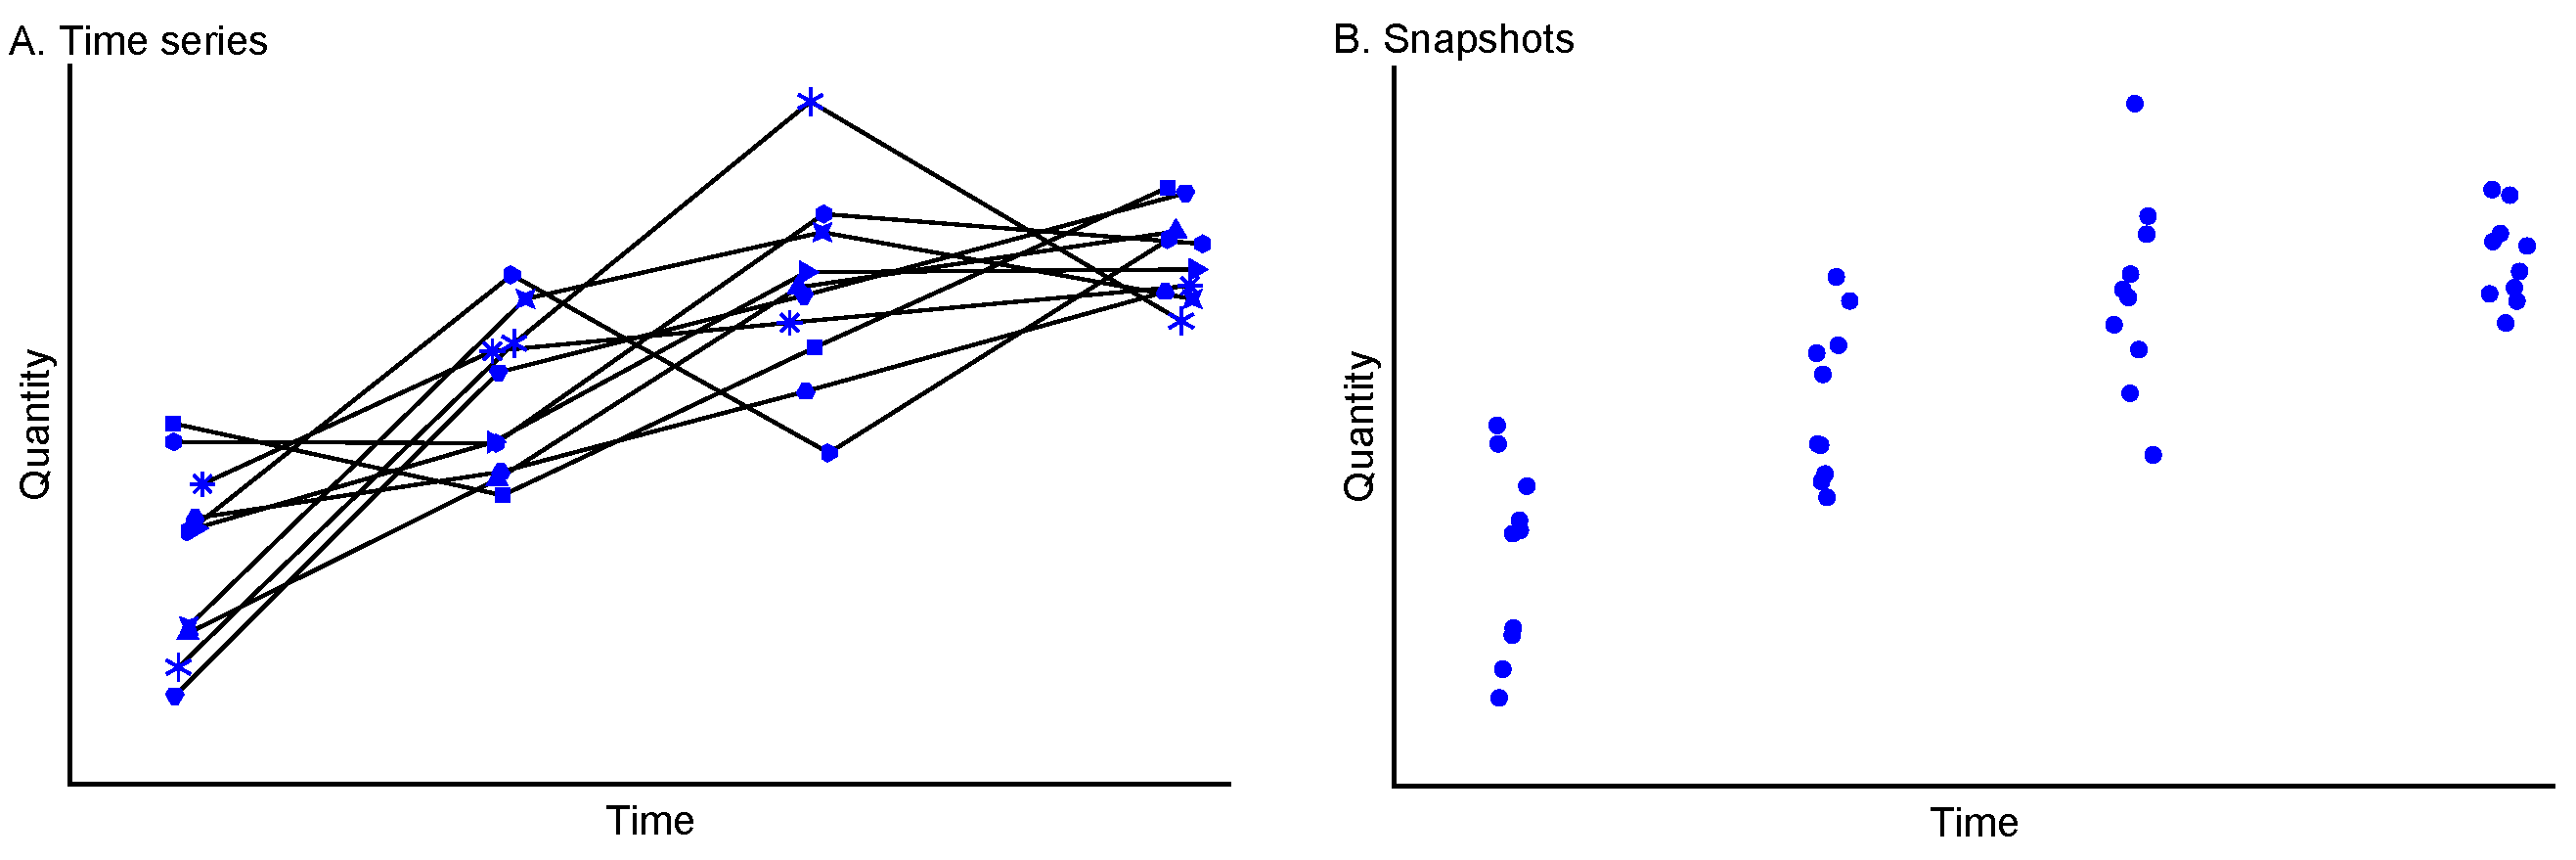
\includegraphics[width=\textwidth]{../figures/time_series_v_snapshots.pdf}}
  \caption{\textbf{Data typical of single cell experiments. (A) Time series data. (B) Snapshot data.} In A, note cell identities are retained at each measurement time (indicated by individual plot markers), whereas in the snapshot data in B, either this information is lost, or more often, cells are destroyed by the measurement process, and each observation corresponds to a distinct cell.}
  \label{fig:time_series_v_snapshots}
\end{figure}

We model the processes of an individual cell using a system of ordinary differential equations (ODEs), where each element of the system typically corresponds to the concentration of a particular species. Our initial value problem is,
%
\begin{equation}\label{eq:ode}
\begin{aligned}
\frac{d\boldsymbol{x}}{dt} &= \boldsymbol{f}(\boldsymbol{x}(t); \, \boldsymbol{\theta}), \quad \boldsymbol{f}: \R^k \times \R^p \mapsto \R^k, \\
\boldsymbol{x}(0) &= \boldsymbol{x}_0.
\end{aligned}
\end{equation}
%
Note that in most circumstances, the initial state of the system, $\boldsymbol{x}(0)$, is unknown, and it can be convenient to include these as elements of $\boldsymbol{\theta}$ to be estimated.

\subsection{Snapshot data}
We assume the variation in snapshots arises due to heterogeneity in the underlying parameters, $\boldsymbol{\theta}$, across cells. Therefore, the evolution of the underlying state of cell $i$ is described by an idiosyncratic ODE,
%
\begin{equation} \label{eq:ode_i}
\begin{aligned}
\frac{d\boldsymbol{x}^{\{i\}}}{dt} &= \boldsymbol{f} \left( \boldsymbol{x}^{\{i\}}(t); \, \boldsymbol{\theta}^{\{i\}} \right),
                                      \quad \boldsymbol{f}: \R^k \times \R^p \mapsto \R^k, \\
\boldsymbol{x}^{\{i\}}(0) &= \boldsymbol{x}_0,
\end{aligned}
\end{equation}
where superscript $^{\{i\}}$ indicates the $i$th cell.
%
The traditional (non-hierarchical) state-space approach to modelling dynamic systems supposes that measurement error introduces stochastic variation in the output (Figure \ref{fig:data_generation}A). Our approach, by contrast, assumes any variation in outputs is solely due to variation in parameter values between cells (Figure \ref{fig:data_generation}B). Whether the assumption of ``perfect'' measurements is reasonable depends on experimental details of the system under investigation, but we argue our method nevertheless provides a useful approximation in cases where the signal to noise ratio is high. \textcolor{blue}{Butler et al (2018) \cite{BJW-18} consider the effect of measurement error through a stability analysis of the posterior distribution and provide a priori bounds on the posterior distributions in theorems 4.1 and 4.5.} \textcolor{blue}{Once again we emphasize that we are considering distributions of quantities of interest with no sense of specific individual trajectories, making a mixed effects modeling approach problematic.}

\begin{figure}[H]
  \centerline{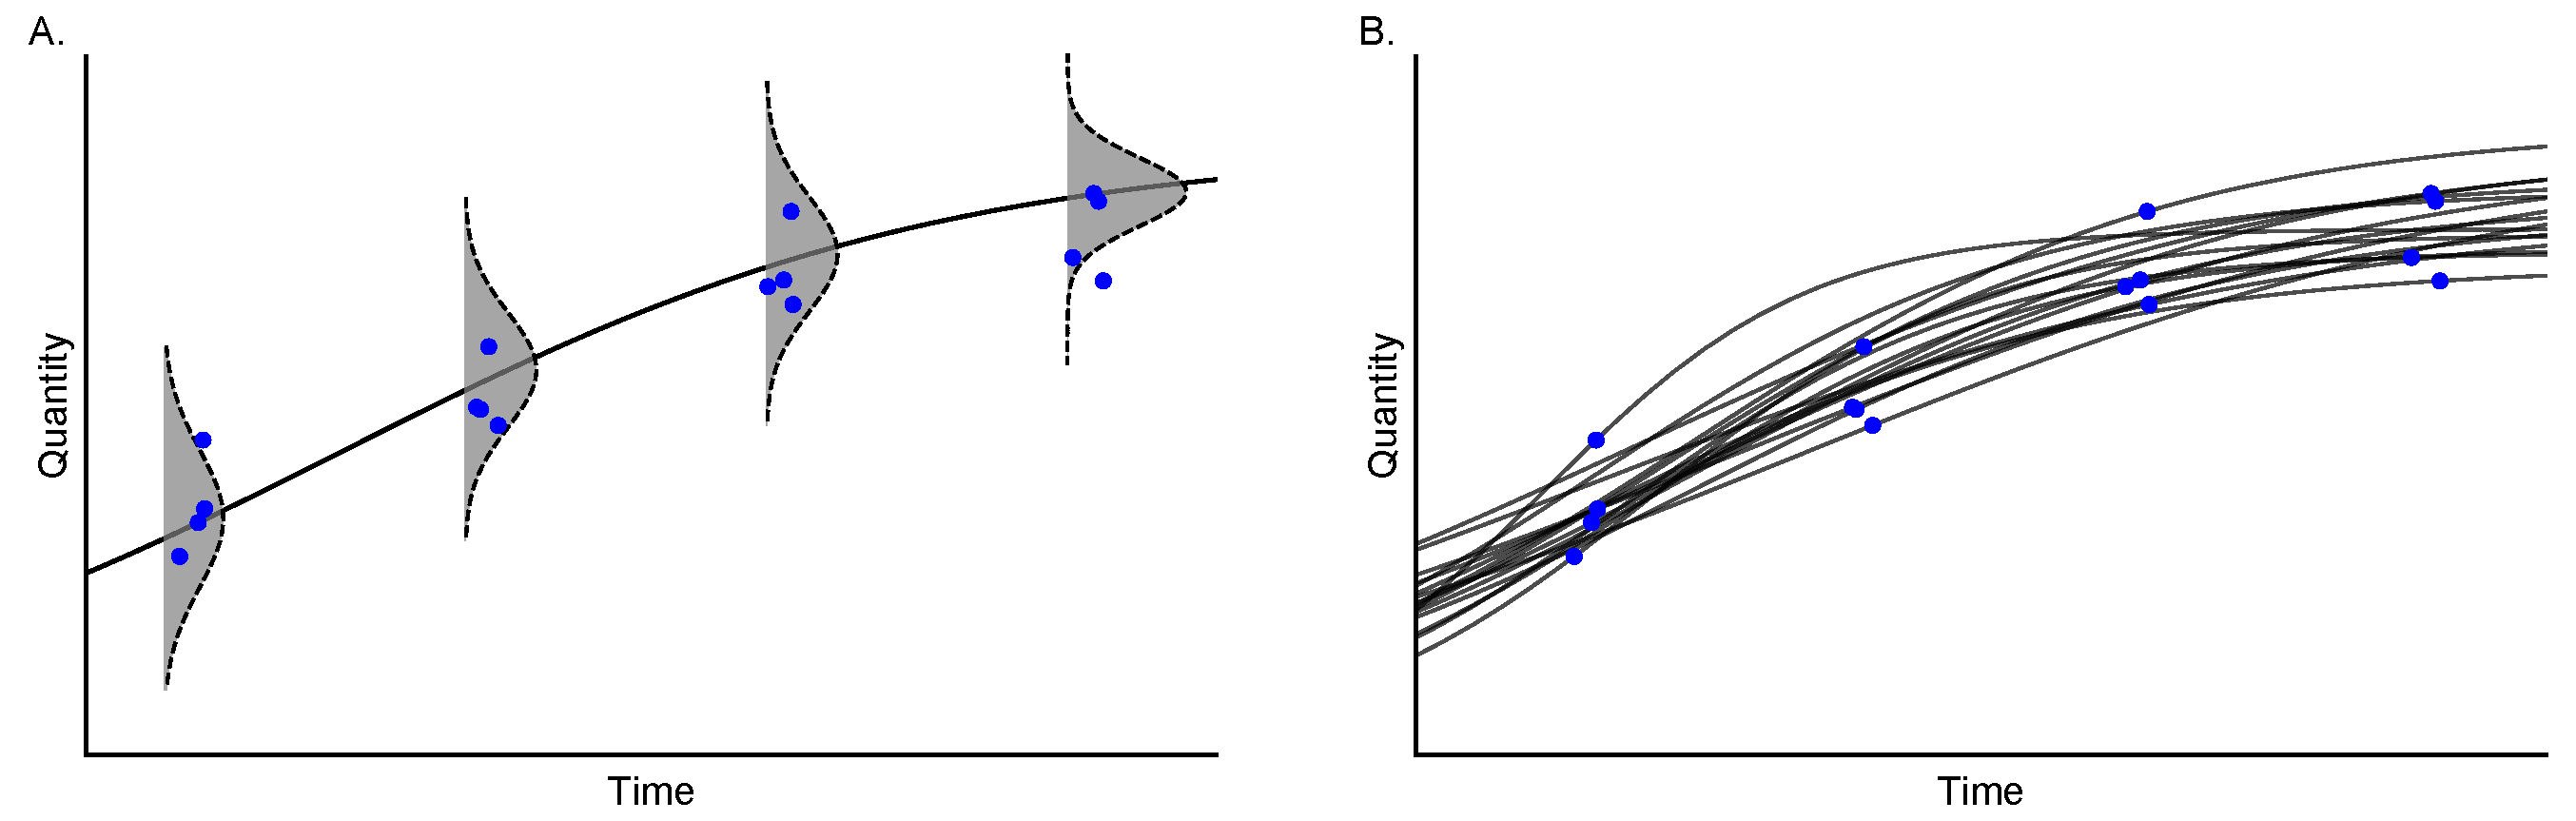
\includegraphics[width=\textwidth]{../figures/data_generation.pdf}}
  \caption{\textbf{Models of variation in observed outputs. (A) State-space model. (B) Parameter heterogeneity model.} (A) For non-hierarchical state-space models , there is a single ``true'' latent state, and observations result from an imperfect measurement process (grey histograms). (B) For models with parameter heterogeneity, the uncertainty is generated by differences in cellular processes (black lines) between cells. Note that, in both cases, individual cells are measured only once in their lifetime.}
  \label{fig:data_generation}
\end{figure}

In an experiment, quantities of interest (QOIs) are measured. Examples of QOIs include concentrations of compounds at different points in time, peak voltages across cell membranes during an action potential, or measurements of cell volume. Here, we suppose $m\geq 1$ QOIs are measured,
%
\begin{equation}
\boldsymbol{q}^\top = \left( q_1, q_2, \dots, q_m \right) \in \R^m,
\end{equation}
%
with $n_j$ observations of each quantity, $q_j$. Distinct QOIs, $q_j$, may correspond to different functionals of the solution at the same time or the same functional at different times. The observed data for QOI $q_j$ at the corresponding time $t_j$ consists of the $n_j$ cellular measurements,
%
\begin{equation}
\boldsymbol{y}(t_j)^\top = \left( q_j(x^{\{1\}}(t_j)), q_j(x^{\{2\}}(t_j)), \dots, q_j(x^{\{n_j\}}(t_j))  \right) \in \R^{n_j}.
\end{equation}
%
The raw snapshot data $\boldsymbol{Y}$ is the collection of all measured QOIs,
%
\begin{equation}
\boldsymbol{Y} = \left( \boldsymbol{y}(t_1), \boldsymbol{y}(t_2), \dots, \boldsymbol{y}(t_m) \right) \in \R^{n_1} \times \R^{n_2}\times...\times\R^{n_m}.
\end{equation}
%
The goal of inference is to characterise the probability distribution $p(\boldsymbol{\theta}|\boldsymbol{Y})$ representing heterogeneity in cellular processes. The numbers of cells sampled in typical experimental setups is large, and, following previous work, we represent snapshot data $\boldsymbol{Y}$ using probability distributions \cite{hasenauer2011identification,hasenauer2014ode,loos2018hierarchical,dixit2018maximum}. In the first step of our workflow (Figure \ref{fig:workflow}(i)), these distributions are approximated by a kernel density model, with support over the space of the QOI vector, $\boldsymbol{q}\in\R^m$. We use $\hat{\Phi}$ to denote the parameter estimates of the corresponding kernel density model, $p(\boldsymbol{q}|\Phi)$, resultant from fitting it to raw snapshot data. We assume there are enough observational data that the estimated probability distributions are approximate sufficient statistics of the posterior distribution, meaning $p(\boldsymbol{\theta}|\hat{\Phi}) \approx p(\boldsymbol{\theta}|\boldsymbol{Y})$.

The aim of our inverse problem, hence, becomes to derive a ``posterior'' parameter distribution, which, when fed through the deterministic transformation described by the model, $\boldsymbol{q}(\boldsymbol{\theta})$, recapitulates the fitted output density,
%
\begin{equation}
p(\boldsymbol{\theta}|\hat{\Phi}) \xrightarrow{\boldsymbol{q}(\boldsymbol{\theta})} p(\boldsymbol{q}|\hat{\Phi}).
\end{equation}
%
In measure theoretic terms, the intrinsic measure implied by $p(\boldsymbol{\theta}|\hat{\Phi})$ is known as the \textit{push forward} of the measure implied by $p(\boldsymbol{\theta}|\hat{\Phi})$ with respect to the model \cite{BJW-18}.


\begin{table}[htbp]
\centering
%\scriptsize
\begin{adjustwidth}{-0.6in}{0in}%
\begin{tabularx}{1.2\textwidth}{lll}
Variable	                                                & Definition                                   & Dimension \\
\toprule
$\boldsymbol{x}(t)$                                     	& ODE solution                                 & $\R^k$ \\
$\boldsymbol{\theta}$                                     	& ODE parameters                               & $\R^p$ \\
$\boldsymbol{f}(\boldsymbol{x}(t); \, \boldsymbol{\theta})$	& ODE RHS                                      & $\R^k$ \\
$\boldsymbol{x}^{\{i\}}(t)$                                 & ODE solution for cell $i$                    & $\R^k$ \\
$q_j= q_j(\boldsymbol{x}(t_j);\boldsymbol{\theta}) = q_j(\boldsymbol{\theta})$                             & quantity of interest (QOI) $j$               & $\R^1$ \\
$\boldsymbol{q}^\top= \left( q_1, \dots, q_m \right)$            & $m$ distinct QOIs                            & $\R^m$ \\
$q_j^{\{i\}}= q_j(\boldsymbol{x}^{\{i\}}(t_j))$             & QOI $j$ for cell $i$                         & $\R^1$ \\
$\boldsymbol{y}_j^\top=\left( q_j^{\{1\}}, \dots q_j^{\{n_j\}} \right)$  & QOI $j$ for cells $1, \dots, n_j$    & $\R^{n_j}$ \\
$\boldsymbol{Y}=(\boldsymbol{y}_1,...,\boldsymbol{y}_m)$    & ``snapshot'' of all QOIs                      & $\R^{n_1} \times \R^{n_2}\times...\times\R^{n_m}$ \\
$\Phi$ & parameters of output target distribution, $p(\boldsymbol{q}|\Phi)$              & $\R^m$ \\
$\Xi$  & parameters of prior parameter distribution, $p(\boldsymbol{\theta}|\Xi)$        & $\R^p$ \\
$\Psi$ & parameters of prior output distribution, $p(\boldsymbol{q}|\Psi)$               & $\R^p$ \\
$\hat{a}$ & estimates of any quantity $a$                                                                  & - \\
$\Omega(\boldsymbol{z})$              & region of parameter space mapping to $\boldsymbol{q}=\boldsymbol{z}$         & $\R^{\leq p}$ \\
$\mathcal{V}(\boldsymbol{z})$         & volume of $\Omega(\boldsymbol{z})$                                 & $\R^+$ \\
$V$                                   & volume of (bounded) parameter space                                          & $\R^+$ \\
$a^{[n]}$ & $n$th sample of any quantity $a$ & -\\
\end{tabularx}
\caption{\textbf{Glossary of variable names used in this paper.}}
\label{tab:variable_glossary}
\end{adjustwidth}
\end{table}




\subsection{Theoretical development of CMC}
We consider the under-determined case where there are fewer QOIs than model parameters ($m<p$). This means that, provided a given QOI can be generated by the model, it can be produced from any member of a subset of parameter space. Unlike the fully-determined case, these subsets (in general) have non-zero ``volume'', and we term them ``iso-output contour regions'' \textcolor{blue}{\cite{butler2014solving}}. Symbolically, we represent the iso-output contour region for a given quantity of interest $\tilde{\boldsymbol{q}}$ (say) by $\Omega(\tilde{\boldsymbol{q}}) = \{\boldsymbol{\theta}: \boldsymbol{q}(\boldsymbol{\theta}) = \tilde{\boldsymbol{q}}\}$.

In general,  contour ``volumes'' $\mathcal{V}(\tilde{\boldsymbol{q}})$  depend on the chosen output value $\tilde{\boldsymbol{q}}$ (Figure \ref{fig:contour_volumes}). Further, the interpretation of these ``volumes'' depends upon their dimensions. For a model with two parameters, iso-output contour regions are one-dimensional lines, whose size is a length; for a model with three parameters, contour regions are surfaces, whose size is an area; for four-dimensional parameter spaces, contour regions are three-dimensional and their size is a volume; and for models with $p>4$ parameters, iso-contour regions are $p-1$ dimensional manifolds, whose size is a hypervolume.

MCMC methods aim to approximate a posterior parameter distribution by sampling from it. In this case, the resultant parameter samples, when pushed through the model, should approximate samples from the desired QOI distribution. Random Walk Metropolis \cite{lambert2018Student} is a ``vanilla'' MCMC sampler which chooses where next to step based on the ratio of probability densities at the proposed parameter value and current position. Using a vanilla sampler for our case, unfortunately, does not work because the Markov chains are biased towards those regions of parameter space with the largest iso-output contour volumes. This bias means that the stationary parameter distribution obtained, when fed through the model, does not recapitulate the target output distribution \cite{lambert2018inverse}.

Sampling algorithms, therefore, need to explicitly account for the differential volume of iso-output contours. In applied problems, however, we do not know the volumes of iso-output contours and they cannot be exactly calculated for all but the simplest models. Instead in CMC, we estimate them. The following analysis provides a brief introduction to a probabilistic formulation of under-determined inverse problems (see our companion paper \cite{lambert2018inverse} for a more comprehensive discussion). In doing so, this suggests a sampling based approach for estimating contour volumes, which are then exploited by our CMC algorithm.

\begin{figure}[H]
	\centerline{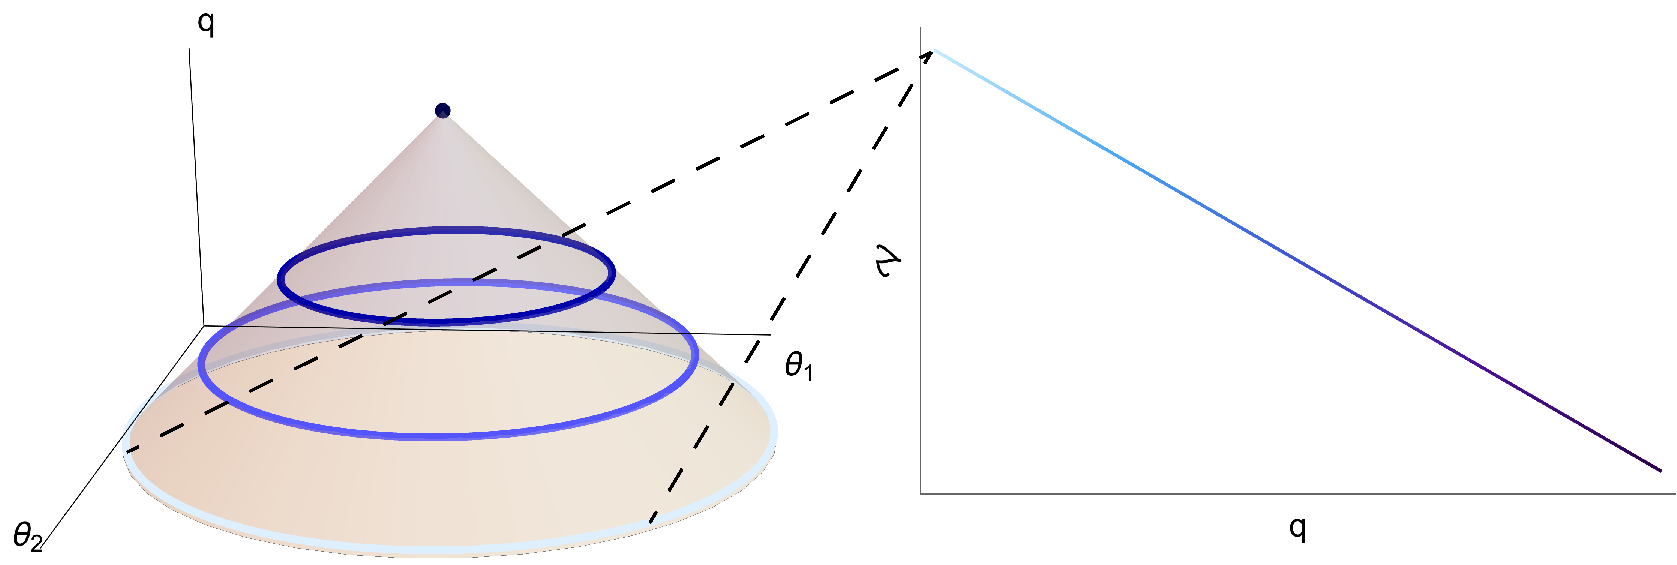
\includegraphics[width=\textwidth]{../figures/contour_volumes_redux.pdf}}
	\caption{\textbf{Left: An example output function $q(\theta_1,\theta_2)$ along with iso-output contours indicated (coloured lines). Right: The ``volume'' of output contours as a function of output value.} Note that here, since parameter space is two dimensional, the ``volume'' of each output value corresponds to a length of an iso-output contour.}
	\label{fig:contour_volumes}
\end{figure}

Solving our inverse problem requires determining the posterior distribution of parameter values, $p(\boldsymbol{\theta}|\hat{\Phi})$, which, when used as input to the forward map, results in the target distribution, $p(\boldsymbol{q}|\hat{\Phi})$. To derive the posterior parameter distribution, we consider the joint density of parameters and QOIs, $p(\boldsymbol{\theta},\boldsymbol{q}|\hat{\Phi})$. This can be decomposed in two ways using the law of conditional probability,
%
\begin{equation}\label{eq:joint}
  p( \boldsymbol{\theta}, \boldsymbol{q}|\hat{\Phi})
= p( \boldsymbol{\theta}|\boldsymbol{q}, \hat{\Phi}) \times p(\boldsymbol{q}|\hat{\Phi})
= p( \boldsymbol{q}|\boldsymbol{\theta}, \hat{\Phi}) \times p(\boldsymbol{\theta}|\hat{\Phi}).
\end{equation}
%
Rearranging eq. (\ref{eq:joint}), we obtain the posterior parameter distribution,
%
\begin{equation}\label{eq:posterior_mid}
p(\boldsymbol{\theta}|\hat{\Phi})
= \frac{p(\boldsymbol{\theta}|\boldsymbol{q}, \hat{\Phi}) \times p(\boldsymbol{q}|\hat{\Phi})}{p(\boldsymbol{q}| \boldsymbol{\theta}, \hat{\Phi})}.
\end{equation}
%
\textcolor{blue}{Note that eq. \eqref{eq:posterior_mid} is only well defined if the denominator is non-zero and for a deterministic map, this occurs only when $\boldsymbol{q}=\boldsymbol{q}(\boldsymbol{\theta})$. (Since the mapping from parameters to outputs is deterministic, $p(\boldsymbol{q}| \boldsymbol{\theta}, \hat{\Phi})=\delta(\boldsymbol{q}(\boldsymbol{\theta}))$, i.e., the Dirac delta function centred at $\boldsymbol{q}=\boldsymbol{q}(\boldsymbol{\theta})$.)  }
 Thus eq. \eqref{eq:posterior_mid} becomes,
%
\begin{equation}\label{eq:posterior_mid1}
p(\boldsymbol{\theta}|\hat{\Phi})
= p(\boldsymbol{\theta}|\boldsymbol{q}(\boldsymbol{\theta}), \hat{\Phi}) \times p(\boldsymbol{q}(\boldsymbol{\theta})|\hat{\Phi}).
\end{equation}
%
In the same way that a single output value can be caused by any member of a set of parameter values, a target output distribution $p(\boldsymbol{q}|\hat{\Phi})$ can be caused by any member of a set of parameter distributions. To ensure uniqueness of the ``posterior'' parameter distributions, we must, therefore, specify ``prior'' distributions for the parameters, as in more traditional Bayesian inference. In what follows, we assume the conditional distribution $p(\boldsymbol{\theta}|\boldsymbol{q}, \hat{\Phi})$ is independent of the data, i.e., $p(\boldsymbol{\theta}|\boldsymbol{q}, \hat{\Phi})=p(\boldsymbol{\theta}|\boldsymbol{q})$, and thus represents a conditional ``prior'' which can be manipulated using Bayes' rule as,
%
\begin{equation}\label{eq:prior}
p(\boldsymbol{\theta}|\boldsymbol{q}(\boldsymbol{\theta})) = \frac{p(\boldsymbol{\theta})}{p(\boldsymbol{q}(\boldsymbol{\theta}))}.
\end{equation}
%
This results in the form of the posterior parameter distribution targeted by our sampling algorithm,
%
\begin{equation}\label{eq:posterior_input}
p(\boldsymbol{\theta}|\hat{\Phi}) = \frac{p(\boldsymbol{\theta})}{p(\boldsymbol{q}(\boldsymbol{\theta}))} p(\boldsymbol{q}(\boldsymbol{\theta})|\hat{\Phi}).
\end{equation}
%
Again, we defer to our companion piece \cite{lambert2018inverse} for detailed explanation of eqs. (\ref{eq:prior}) and (\ref{eq:posterior_input}) and, instead, here provide brief interpretation when considering a uniform prior on parameter space. In this case, $p(\boldsymbol{\theta}) = \frac{1}{V}$, where $V$ is the total volume of parameter space. The denominator term of eq. (\ref{eq:prior}) is the prior induced on output space by the prior over parameter space. For a uniform prior on parameter values, this is,
%
\begin{equation}\label{eq:contour_volume}
p(\boldsymbol{\theta}|\boldsymbol{q}(\boldsymbol{\theta})) = \frac{1}{\mathcal{V}(\boldsymbol{q}(\boldsymbol{\theta}))},
\end{equation}
%
where $\mathcal{V}(\boldsymbol{q}(\boldsymbol{\theta}))$ is the volume of parameter space occupied by the iso-output contour $\Omega(\boldsymbol{q}(\boldsymbol{\theta}))$ (see Fig. \ref{fig:contour_volumes} for the meaning of this volume for a two parameter example). Therefore, a uniform prior over parameter space implies a prior structure where all parameter values producing the same output are given equal weighting.

\subsection{Implementation of CMC}

Except for some toy examples, the denominator of eq. (\ref{eq:prior}) cannot be calculated, so exact sampling from the posterior parameter distribution of eq. (\ref{eq:posterior_input}) is not, in general, possible. We propose, instead, a computationally efficient sampling method to estimate $p(\boldsymbol{q}(\boldsymbol{\theta}))$, which forms the first step of our so-called ``Contour Monte Carlo'' (CMC) algorithm (Algorithm \ref{alg:cmc}; Figure \ref{fig:workflow}(ii)), where the volume of iso-output contours with each feasible output value is estimated. This step involves repeated independent sampling from the prior distribution of parameters, $\boldsymbol{\theta}^{[i]}\sim p(\boldsymbol{\theta}|\Xi)$, where $\Xi$ parameterises the prior probability density.
Each parameter sample is then mapped to an output value, $\boldsymbol{q}^{[i]}=\boldsymbol{q}(\boldsymbol{\theta}^{[i]})$. The collection of output samples is then fitted using a vine copula kernel density estimator (KDE) \cite{nagler2016evading}, $\hat{\Psi} = \argmax_\Psi p\left(\left( \boldsymbol{q}^{[1]}, \dots ,\boldsymbol{q}^{[N_1]} \right)|\Psi\right)$. Throughout the course of development of CMC, we have tested many KDE methods and have found vine copula KDE is best suited to approximating the higher dimensional probability distributions required in practice.


The second step in our algorithm then uses MCMC to sample from an approximate version of eq. (\ref{eq:posterior_input}), where the estimated density, $p(\boldsymbol{q}(\boldsymbol{\theta})|\hat{\Psi})$ replaces its corresponding estimand (Algorithm \ref{alg:cmc}; Figure \ref{fig:workflow}(iii)),
%
\begin{equation}\label{eq:posterior_input_estimated}
p(\boldsymbol{\theta}|\hat{\Phi},\Xi,\hat{\Psi}) =
\frac{p(\boldsymbol{\theta}|\Xi)}{p(\boldsymbol{q}(\boldsymbol{\theta})|\hat{\Psi})} \,
p(\boldsymbol{q}(\boldsymbol{\theta})|\hat{\Phi}).
\end{equation}
%
The final step in CMC is to compare output samples generated by MCMC with the target distribution (Figure \ref{fig:workflow}(iv)). Asymptotically (in terms of the sample size of both sampling steps), CMC produces a sample of parameter values $(\boldsymbol{\theta}^{[1]},\boldsymbol{\theta}^{[2]},...)$ which, when mapped to the output space, corresponds to the target distribution $p(\boldsymbol{q}|\hat{\Psi})$. In developing CMC, we found that a finite sample of modest size for both steps of CMC results in parameter samples that, when transformed, often represented good approximations of the target. There are, however, occasions when this is not the case, and this final confirmatory step is indispensable since it frequently highlights inadequacies in contour volume estimation or MCMC, meaning more samples from either or both of these steps are required. It may also be necessary to tweak hyperparameters of the KDE in the contour volume estimation step to ensure reasonable approximation of the distribution of output values obtained by sampling the prior density. If the target distribution is sensitive to the contour volume estimates, this may also indicate that the target snapshot distribution is incompatible with the model: here, we make no claims on existence of a solution to the inverse problem, only that, Contour Monte Carlo is a pragmatic approach to approximate it by sampling if one should exist. A useful way to diagnose whether the target distribution can be produced from the model and chosen priors is to plot the output values from the contour volume estimation step of CMC - this is akin to visualising the prior predictive distribution in traditional Bayesian inference \cite{lambert2018Student}. If the bulk of target probability mass does not overlap with the simulated output values, then the model and/or chosen prior are unlikely to be invertible to this particular target.

\subsection{Workflow and CMC algorithm}

A graphical illustration of the complete CMC workflow is provided in Figure \ref{fig:workflow}. All variables are defined in Table \ref{tab:variable_glossary}. The CMC algorithm is provided in Algorithm \ref{alg:cmc}. In this implementation, MCMC sampling is performed via the Random Walk Metropolis algorithm, but for the examples in \S \ref{sec:results}, we use an adaptive MCMC algorithm \cite{johnstone2016uncertainty}.

\begin{figure}[H]
  \centerline{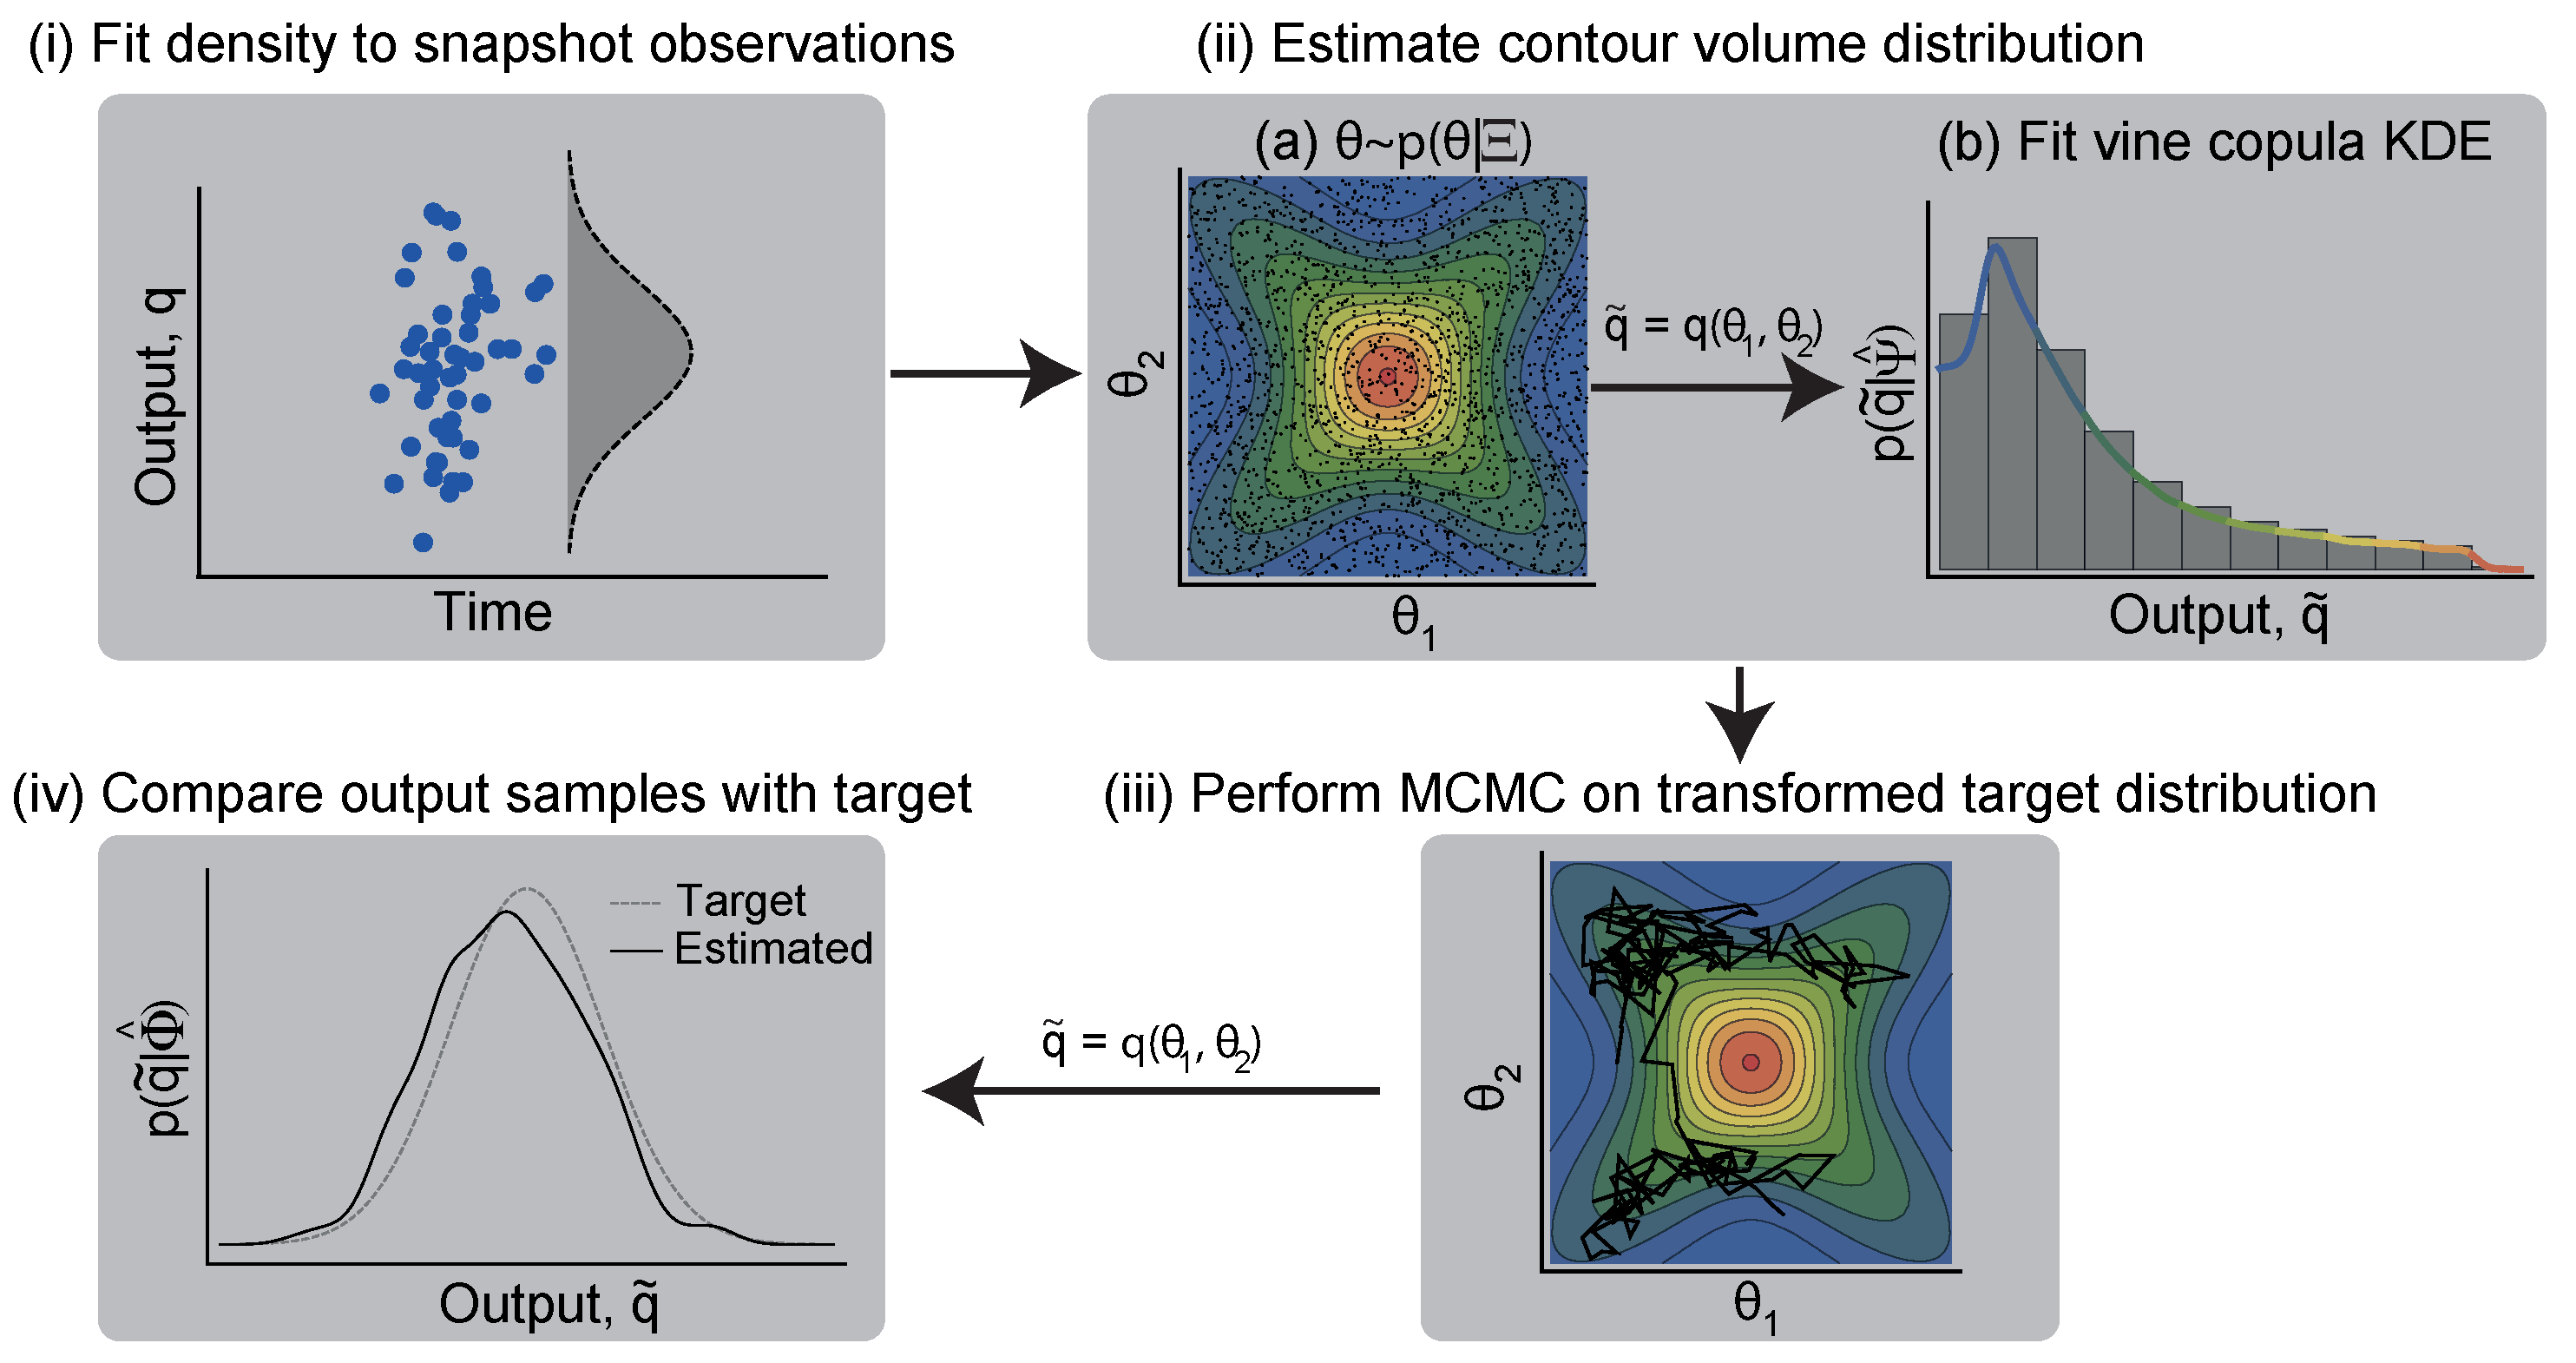
\includegraphics[width=1.5\textwidth]{../figures/workflow.pdf}}
  \caption{\textbf{Workflow for Contour Monte Carlo to estimate cell population heterogeneity.} The distribution targeted in (iii) is given by eq. (\ref{eq:posterior_input_estimated}). Here, $\tilde q$ is used to represent an output value resultant from applying the functional $q$ to parameter samples $(\theta_1,\theta_2)$.}
  \label{fig:workflow}
\end{figure}

\begin{algorithm}[H]
\footnotesize
\texttt{\\}
\begin{algorithmic}
\Procedure{CMC}{$\boldsymbol{Y}, \Xi, N_1, N_2$}\Comment{Sample from posterior parameter distribution}
	\State $\hat{\Phi} = \Call{SnapshotEstimator}{\boldsymbol{Y}}$
	\State $\hat{\Psi} = \Call{ContourVolumeEstimator}{\Xi,N_1}$
	\State $\left(\boldsymbol{\theta}^{[1]},...,\boldsymbol{\theta}^{[N_2]}\right) = \Call{MCMC}{\hat{\Phi},\Xi, \hat{\Psi},N_2}$
	\State $\text{converged} = \Call{CompareOutputToTarget}{(\boldsymbol{\theta}^{[1]},...,\boldsymbol{\theta}^{[N_2]}), \hat{\Phi}}$
	\While{converged$\neq$1} \Comment{Rerun contour volume estimation (if necessary modify vine copula KDE hyperparmeters) and/or MCMC, with larger sample sizes if required}
		 \State $\hat{\Psi}=\Call{ContourVolumeEstimator}{\Xi, N_1'},\; N_1' \geq N_1$
         \State $\left( \boldsymbol{\theta}^{[1]},...,\boldsymbol{\theta}^{[N_2']} \right)
                = \Call{MCMC}{\hat{\Phi},\Xi, \hat{\Psi},N_2'}, \; N_2' \geq N_2$
          \State $\text{converged} = \Call{CompareOutputToTarget}{(\boldsymbol{\theta}^{[1]},...,\boldsymbol{\theta}^{[N_2']} ), \hat{\Phi}}$
          \State $N_1 \leftarrow N_1', \; N_2 \leftarrow N_2'$
	\EndWhile
	\State \Return $\left( \boldsymbol{\theta}^{[1]},...,\boldsymbol{\theta}^{[N_2]} \right)$
\EndProcedure
\end{algorithmic}

\texttt{\\}
\begin{algorithmic}
\Procedure{SnapshotEstimator}{$\boldsymbol{Y}$}\Comment{Fit snapshots with kernel density estimator (KDE)}
	\State $\hat{\Phi} = \argmax_\Phi p(\boldsymbol{Y}|\Phi)$
	\State \Return $\hat{\Phi}$
\EndProcedure
\end{algorithmic}
	
\texttt{\\}
\begin{algorithmic}
\Procedure{ContourVolumeEstimator}{$\Xi, N_1$}\Comment{Estimate volume of contours}
	\For{$i$ in $1:N_1$}
		\State $\boldsymbol{\theta}^{[i]} \sim p(\boldsymbol{\theta}|\Xi)$           \Comment{Sample from prior density}
		\State $\boldsymbol{q}^{[i]} = \boldsymbol{q}(\boldsymbol{\theta}^{[i]})$  \Comment{Calculate corresponding output value}
	\EndFor
	\State $ \hat{\Psi} = \argmax_\Psi p\left(\left( \boldsymbol{q}^{[1]}, \dots ,\boldsymbol{q}^{[N_1]} \right)|\Psi\right)$
           \Comment{Fit vine copula KDE}
	\State \Return $\hat{\Psi}$
\EndProcedure
\end{algorithmic}

\texttt{\\}
\begin{algorithmic}
\Procedure{MCMC}{$\hat{\Phi},\Xi, \hat{\Psi}, N_2$}\Comment{Random Walk Metropolis algorithm targeting posterior parameter distribution}
	\State $\boldsymbol{\theta}^{[0]} \sim \pi(.)$ \Comment{Sample from arbitrary initialisation distribution}
	\For{$i$ in $1:N_2$}
		\State $\boldsymbol{\theta}^{[i]^\prime}\sim \mathcal{N}(\boldsymbol{\theta}^{[i-1]},\boldsymbol{\Sigma})$ \Comment{Propose new parameter values}
		\State
		\Comment{Calculate Metropolis acceptance ratio}
		\State $r =
                     p(\boldsymbol{\theta}^{[i]^\prime}|\Xi) \
                     p(\boldsymbol{q}(\boldsymbol{\theta}^{[i-1]})|\hat{\Psi}) \
                     p(\boldsymbol{q}(\boldsymbol{\theta}^{[i]^\prime})|\hat{\Phi})
                     /
                     \left[
                     p(\boldsymbol{\theta}^{[i-1]}|\Xi) \
                     p(\boldsymbol{q}(\boldsymbol{\theta}^{[i]^\prime})|\hat{\Psi}) \
                     p(\boldsymbol{q}(\boldsymbol{\theta}^{[i-1]})|\hat{\Phi})
                     \right]$
		\State $u\sim U(0,1)$ \Comment{Sample from uniform distribution}
		\If{$r > u$}
		    \State $\boldsymbol{\theta}^{[i]} = \boldsymbol{\theta}^{[i]^\prime}$ \Comment{Accept proposal}
		\Else
		    \State $\boldsymbol{\theta}^{[i]} = \boldsymbol{\theta}^{[i-1]}$ \Comment{Reject proposal}
		\EndIf
	\EndFor
	\State \Return $\left( \boldsymbol{\theta}^{[1]},...,\boldsymbol{\theta}^{[N_2]} \right)$
\EndProcedure
\end{algorithmic}

\texttt{\\}
\begin{algorithmic}
\Procedure{CompareOutputToTarget}{$(\boldsymbol{\theta}^{[1]},...,\boldsymbol{\theta}^{[N_2]}), \hat{\Phi}$}\Comment{Check output distribution close to target}
	\For{$i$ in $1:N_2$}
		\State $\tilde{\boldsymbol{q}}^{[i]} = \boldsymbol{q}(\boldsymbol{\theta}^{[i]})$ \Comment{Compute QOIs for each parameter sample}
	\EndFor
	\If{$ p(\tilde{\boldsymbol{q}}) \approx p(\tilde{\boldsymbol{q}}|\hat{\Phi})?$} \Comment{Compare sampled output distribution with target}
		\State \Return 1 \Comment{If sufficiently close then converged}
	\Else
		\State \Return 0
	\EndIf
\EndProcedure
\end{algorithmic}

\caption{Pseudocode for the Contour Monte Carlo algorithm for sampling from the posterior parameter distribution of eq. (\ref{eq:posterior_input_estimated}). }\label{alg:cmc}
\end{algorithm}

To generate our results in \S\ref{sec:results}, we assumed for the contour volume estimation step sample sizes were sufficient if the output samples from MCMC provided a reasonable approximation to the target, although we recognise that future work should refine this process further. For the MCMC step, we used adaptive covariance MCMC (see SOM of \cite{johnstone2016uncertainty}) to sample from the target distribution, as it typically provides a considerable speed-up over Random Walk Metropolis \cite{metropolis1953equation,lambert2018Student}. We also used the Gelman-Rubin convergence statistic, $\hat{R}$, to diagnose convergence \cite{lambert2018Student,gelman1992inference}, with a convergence threshold of $\hat{R}\leq\sim 1.1$.

To solve the forward model of each differential equation, we used Julia's inbuilt ``solve'' method for ODE models, which automatically chooses an efficient inbuilt solver \cite{bezanson2017julia}. To replicate the results in this section, we recommend readers execute the corresponding Julia scripts (one for each result section) at \url{https://github.com/ben18785/inverse-sensitivity/tree/master/examples}. Note that, these scripts use the ``\textit{RCall}'' library for Julia \cite{batesRCall}, which calls \textsf{R} from Julia. This package was necessary to use the ``\textit{kdevine}'' \textsf{R} package for vine copula kernel density estimation \cite{naglerkdevine2018}.
